%%%%%%%%%%%%%%%%%%%%%%%%%%%%%%%%%%%%%%%%%%%%%%%%%%%%%%%%%%%%%%%%%%%%%%%%%%%%%%%%%%%%%%%%%%%%%%%%%%%%
% ==================================================================================================
% --------------------------------------------------------------------------------------------------
\chapter{Implementation}
This appendix contains implementation details.
%%%%%%%%%%%%%%%%%%%%%%%%%%%%%%%%%%%%%%%%%%%%%%%%%%%%%%%%%%%%%%%%%%%%%%%%%%%%%%%%%%%%%%%%%%%%%%%%%%%%
\section{Computing}
All computation in the current work was performed using the following workstation and software:
\begin{itemize}[topsep=0pt,itemsep=0pt]
  \item \textbf{CPU:} Intel Core i7-6700K 4.00 GHz
  \item \textbf{RAM:} 16.0 GB DDR4
  \item \textbf{GPU:} NVIDIA GeForce GTX 980 Ti
  \item \textbf{OS:} Windows 10 Pro
  \item \textbf{Code:} MATLAB R2011a
\end{itemize}
%%%%%%%%%%%%%%%%%%%%%%%%%%%%%%%%%%%%%%%%%%%%%%%%%%%%%%%%%%%%%%%%%%%%%%%%%%%%%%%%%%%%%%%%%%%%%%%%%%%%
\section{Manual Segmentations}
It was necessary to create and edit a small number of binary segmentation masks during this work. To do this, the Editor module from the 3D Slicer imaging platform \cite{Fedorov2012} was used\footnote{3D Slicer Editor tool documentation is available here: \hreftt{https://www.slicer.org/wiki/Documentation/4.6/Modules/Editor}.}, including the Wand, Paint, and Erase functions. Figure \ref{fig:m08-rev-slicer} shows the user interface during a lesion segmentation.
\begin{figure}[h]
  \centering
  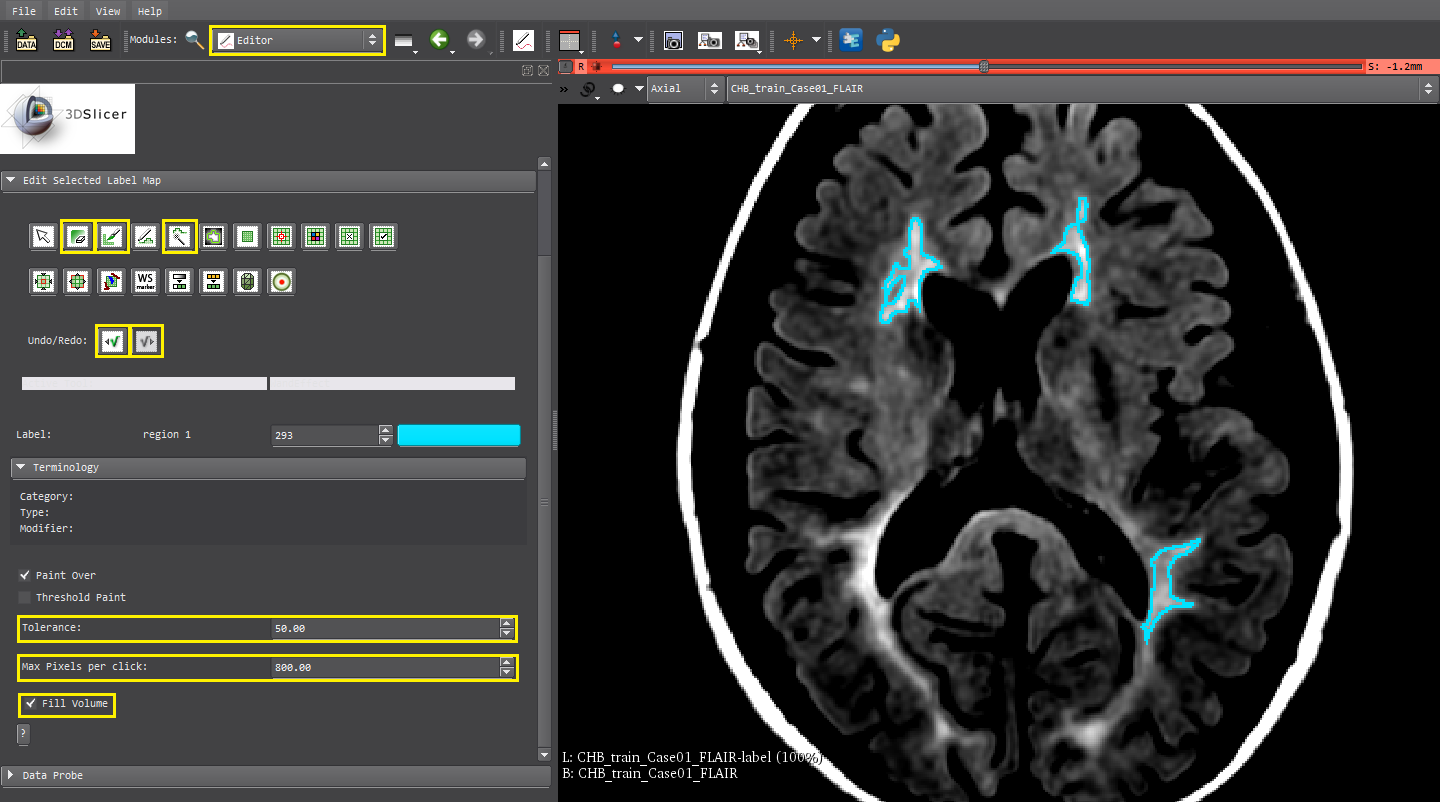
\includegraphics[width=\textwidth]{m08rev-slicer.png}
  \caption{3D Slicer user interface for performing in-house manual segmentations and revisions. The tools used are highlighted in yellow, while the segmentation (in-progress) is shown in blue.}
  \label{fig:m08-rev-slicer}
\end{figure}
% ==================================================================================================
\subsection{MS 2008 WMH Masks}\label{ss:m08-rev}
Since the reported performance of an automatic segmentation algorithm depends on the manual segmentations to which it is compared, it is important to obtain good manual segmentations. Unfortunately, the original manuals in the MS 2008 Segmentation Challenge contained obvious artifacts and inconsistencies, as shown at left in Figure \ref{fig:m08-rev}. Therefore, it was deemed necessary to redo these manuals. The resulting revisions are shown at right in Figure \ref{fig:m08-rev}.
\begin{figure}
  \centering
  \begin{minipage}{6cm}
    \begin{subfigure}{\textwidth}
      \centering\subcaption{Original}\label{fig:m08-rev-o}
      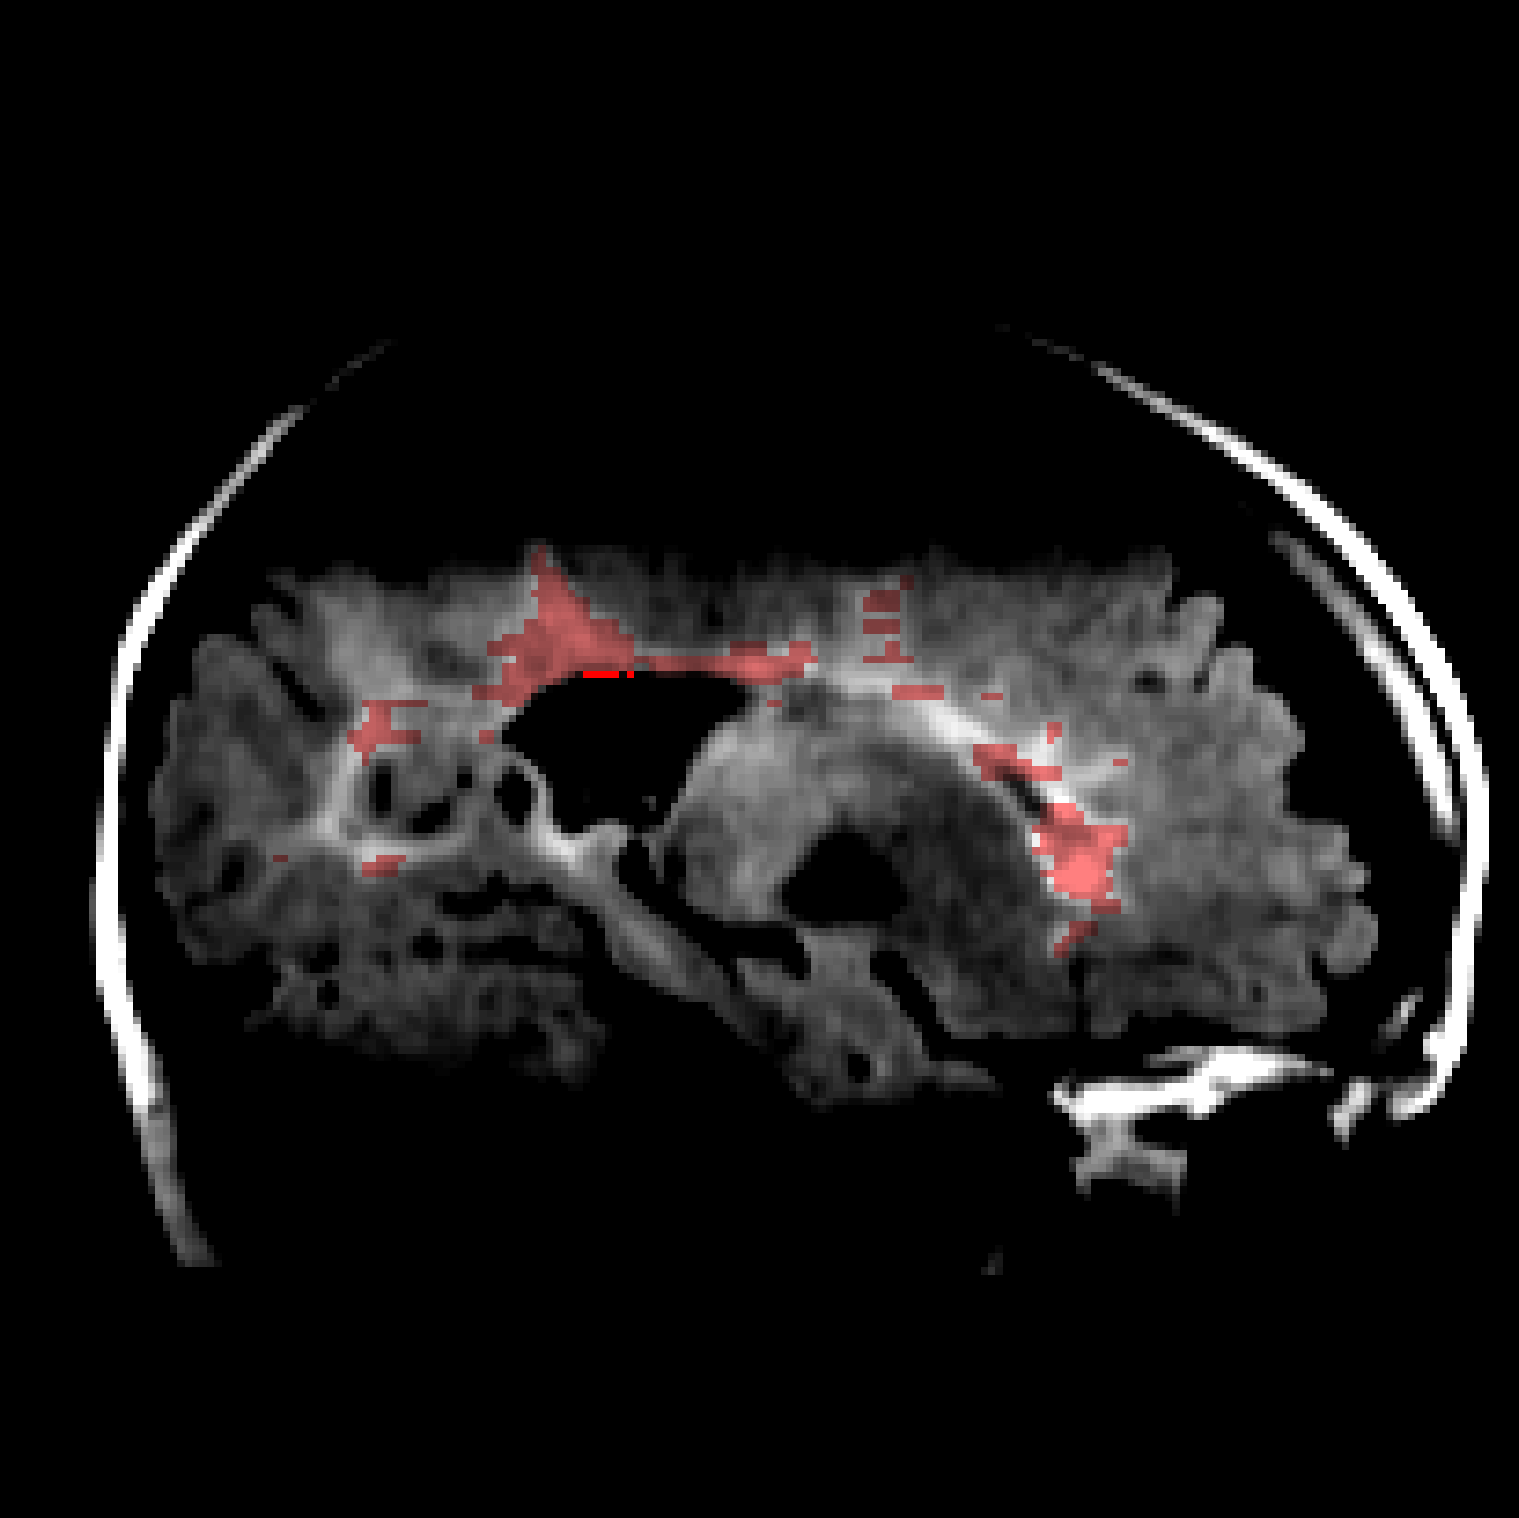
\includegraphics[height=6cm]{m08rev-01-d2-z146-o}\\[0.2em]
      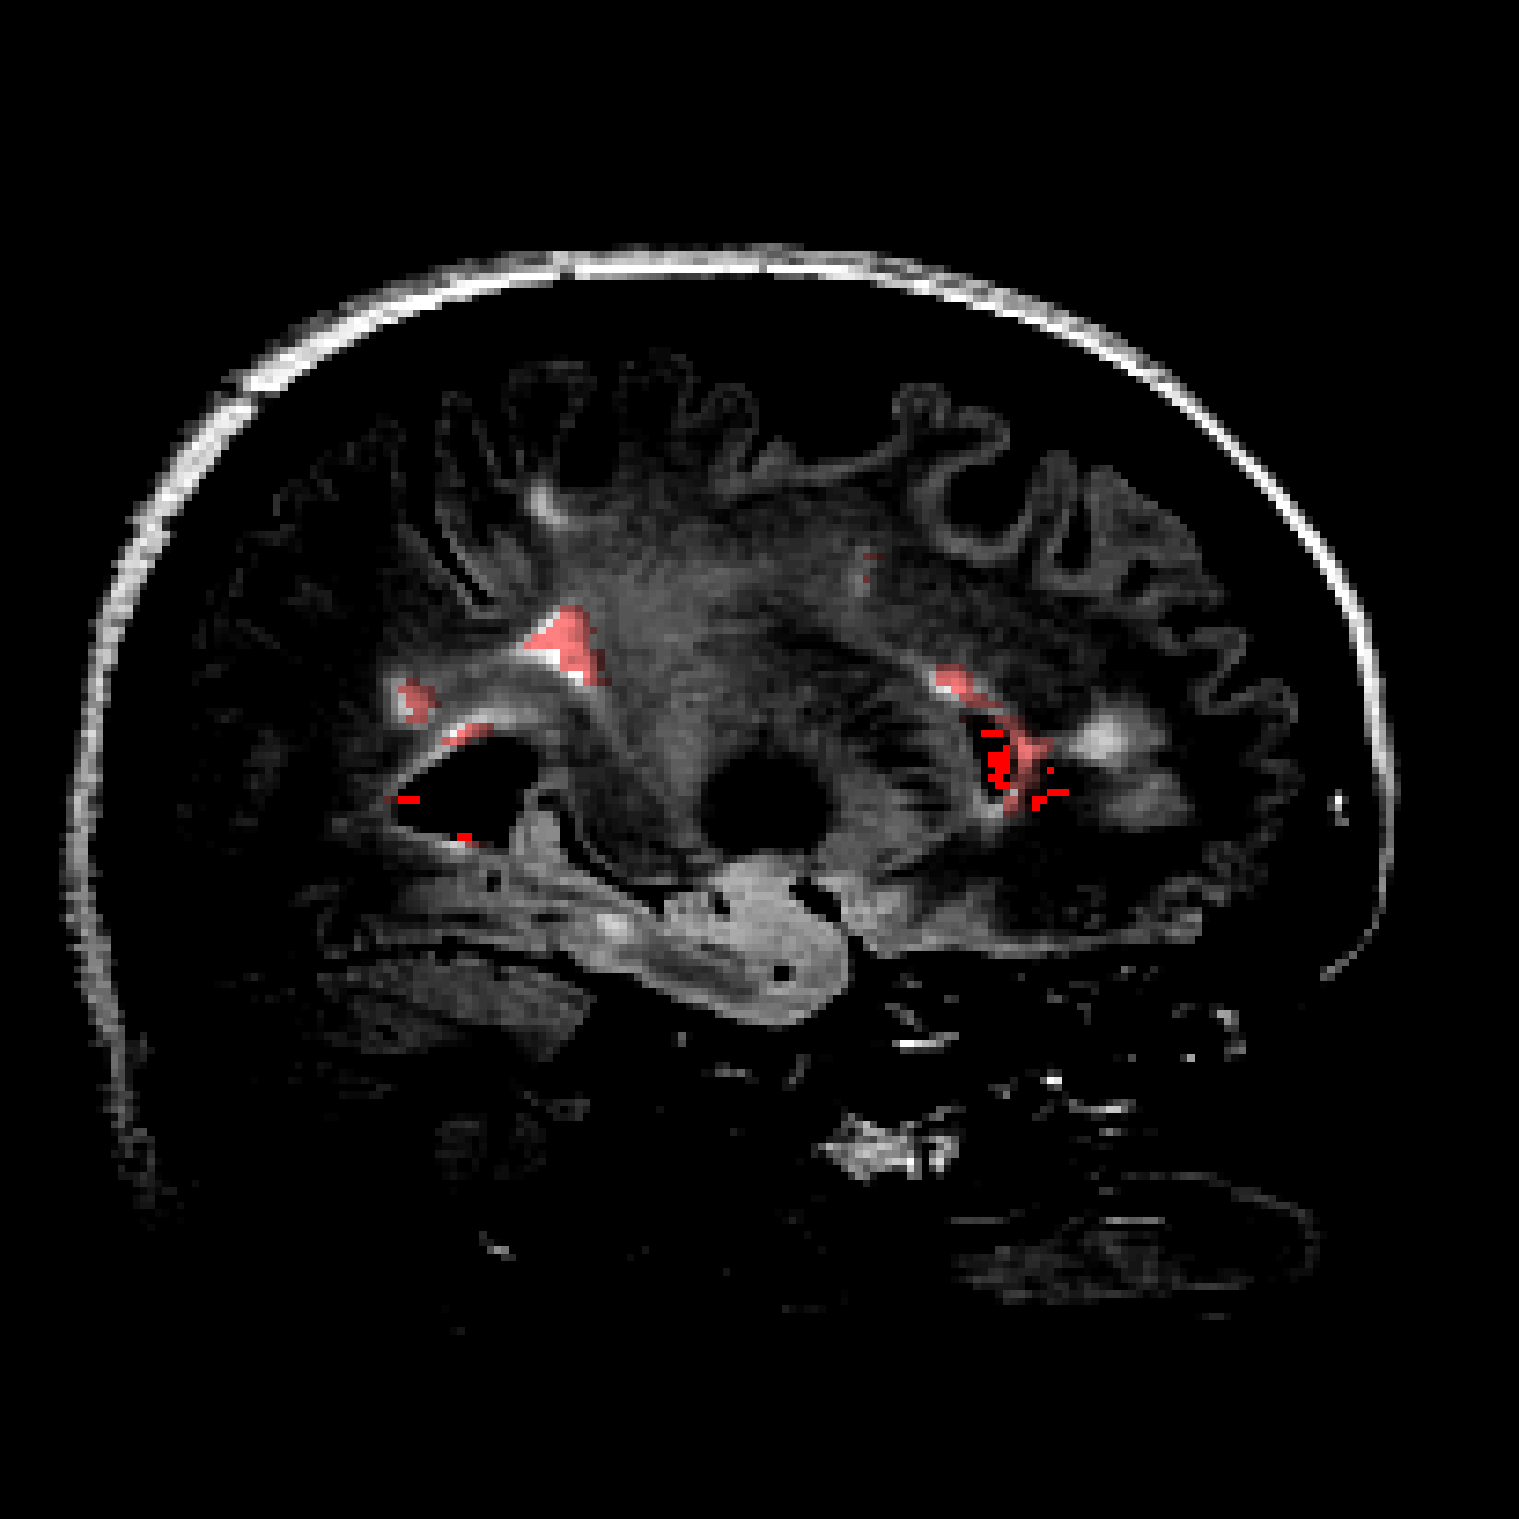
\includegraphics[height=6cm]{m08rev-05-d2-z107-o}\\[0.2em]
      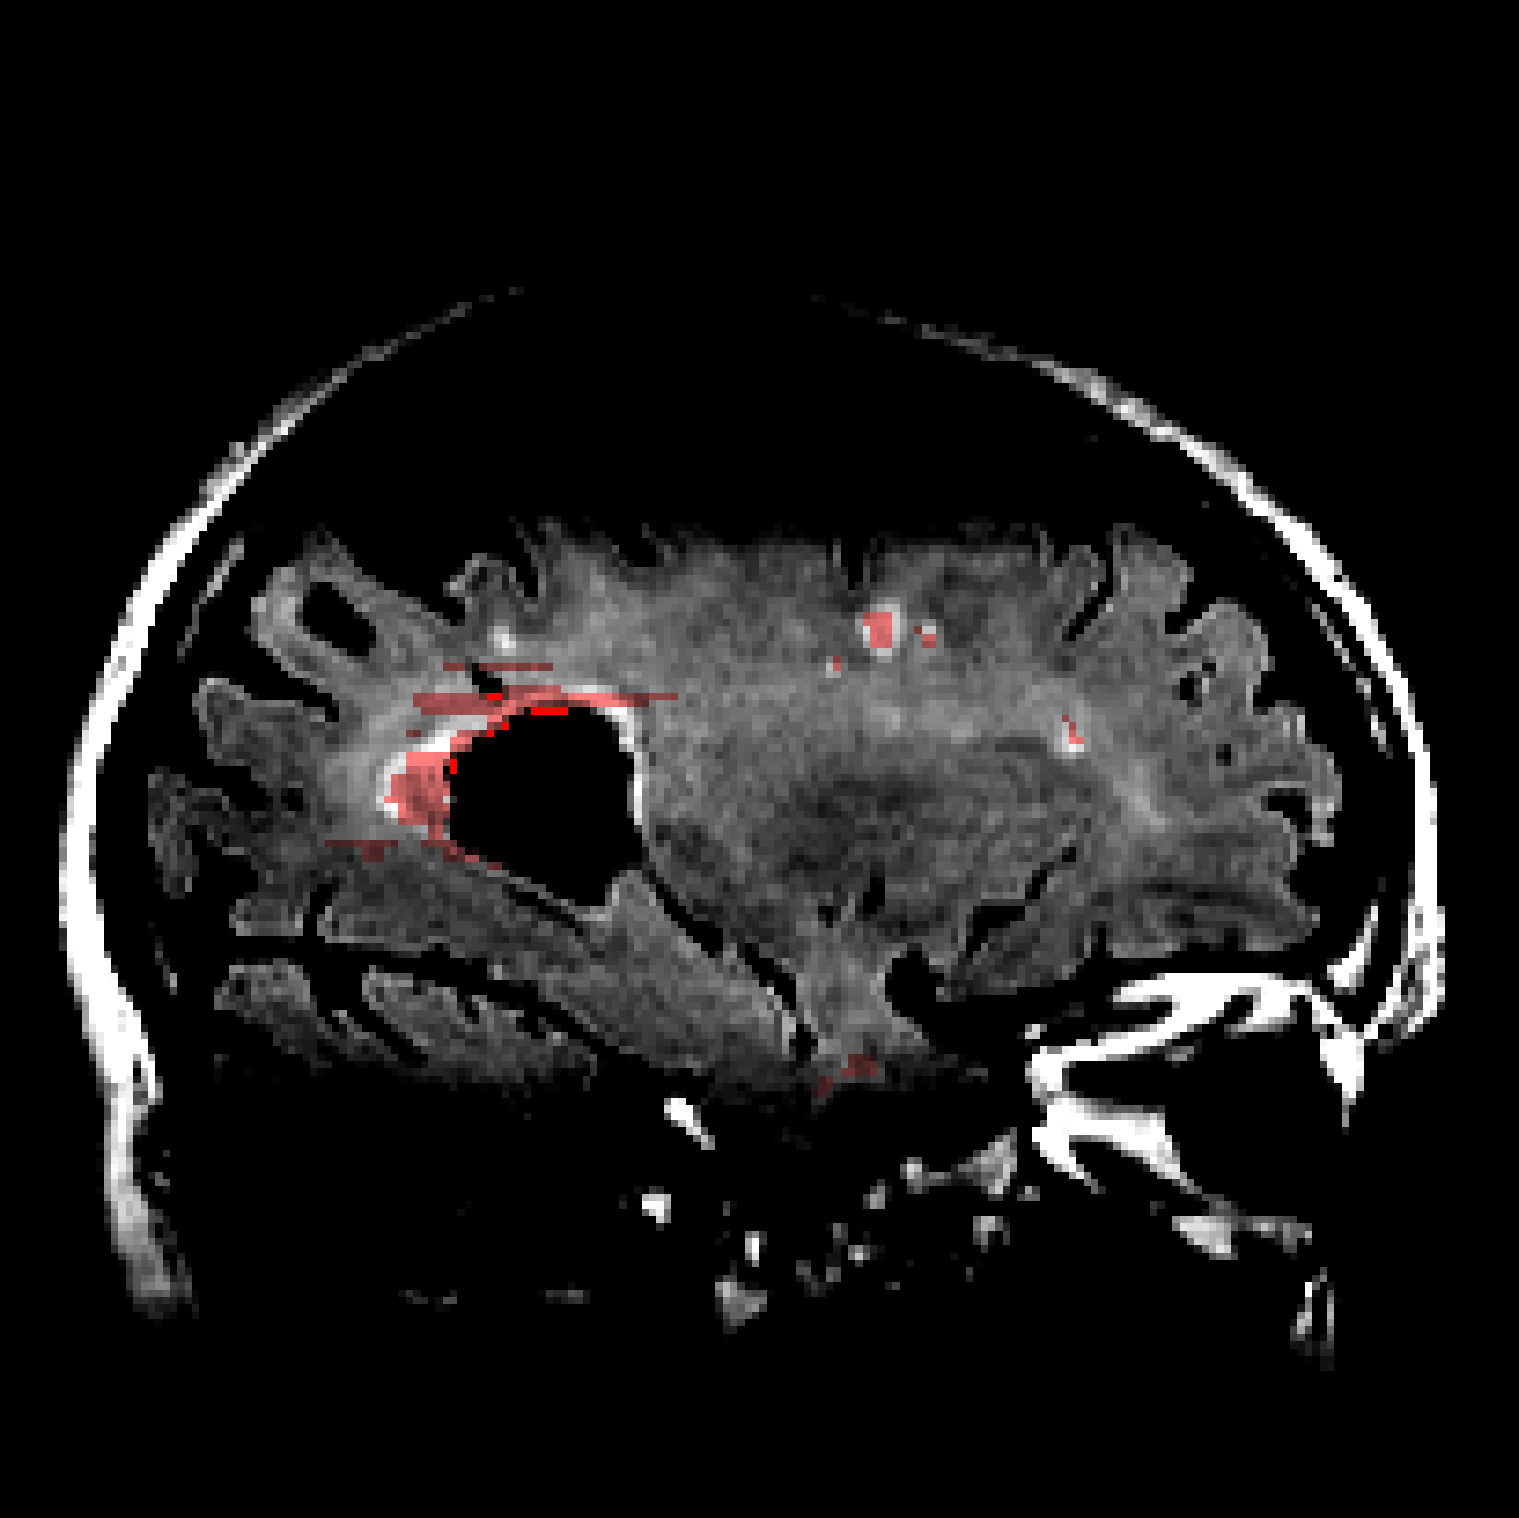
\includegraphics[height=6cm]{m08rev-06-d2-z101-o}
    \end{subfigure}
  \end{minipage}
  \begin{minipage}{6cm}
    \begin{subfigure}{\textwidth}
      \centering\subcaption{Revision}\label{fig:m08-rev-r}
      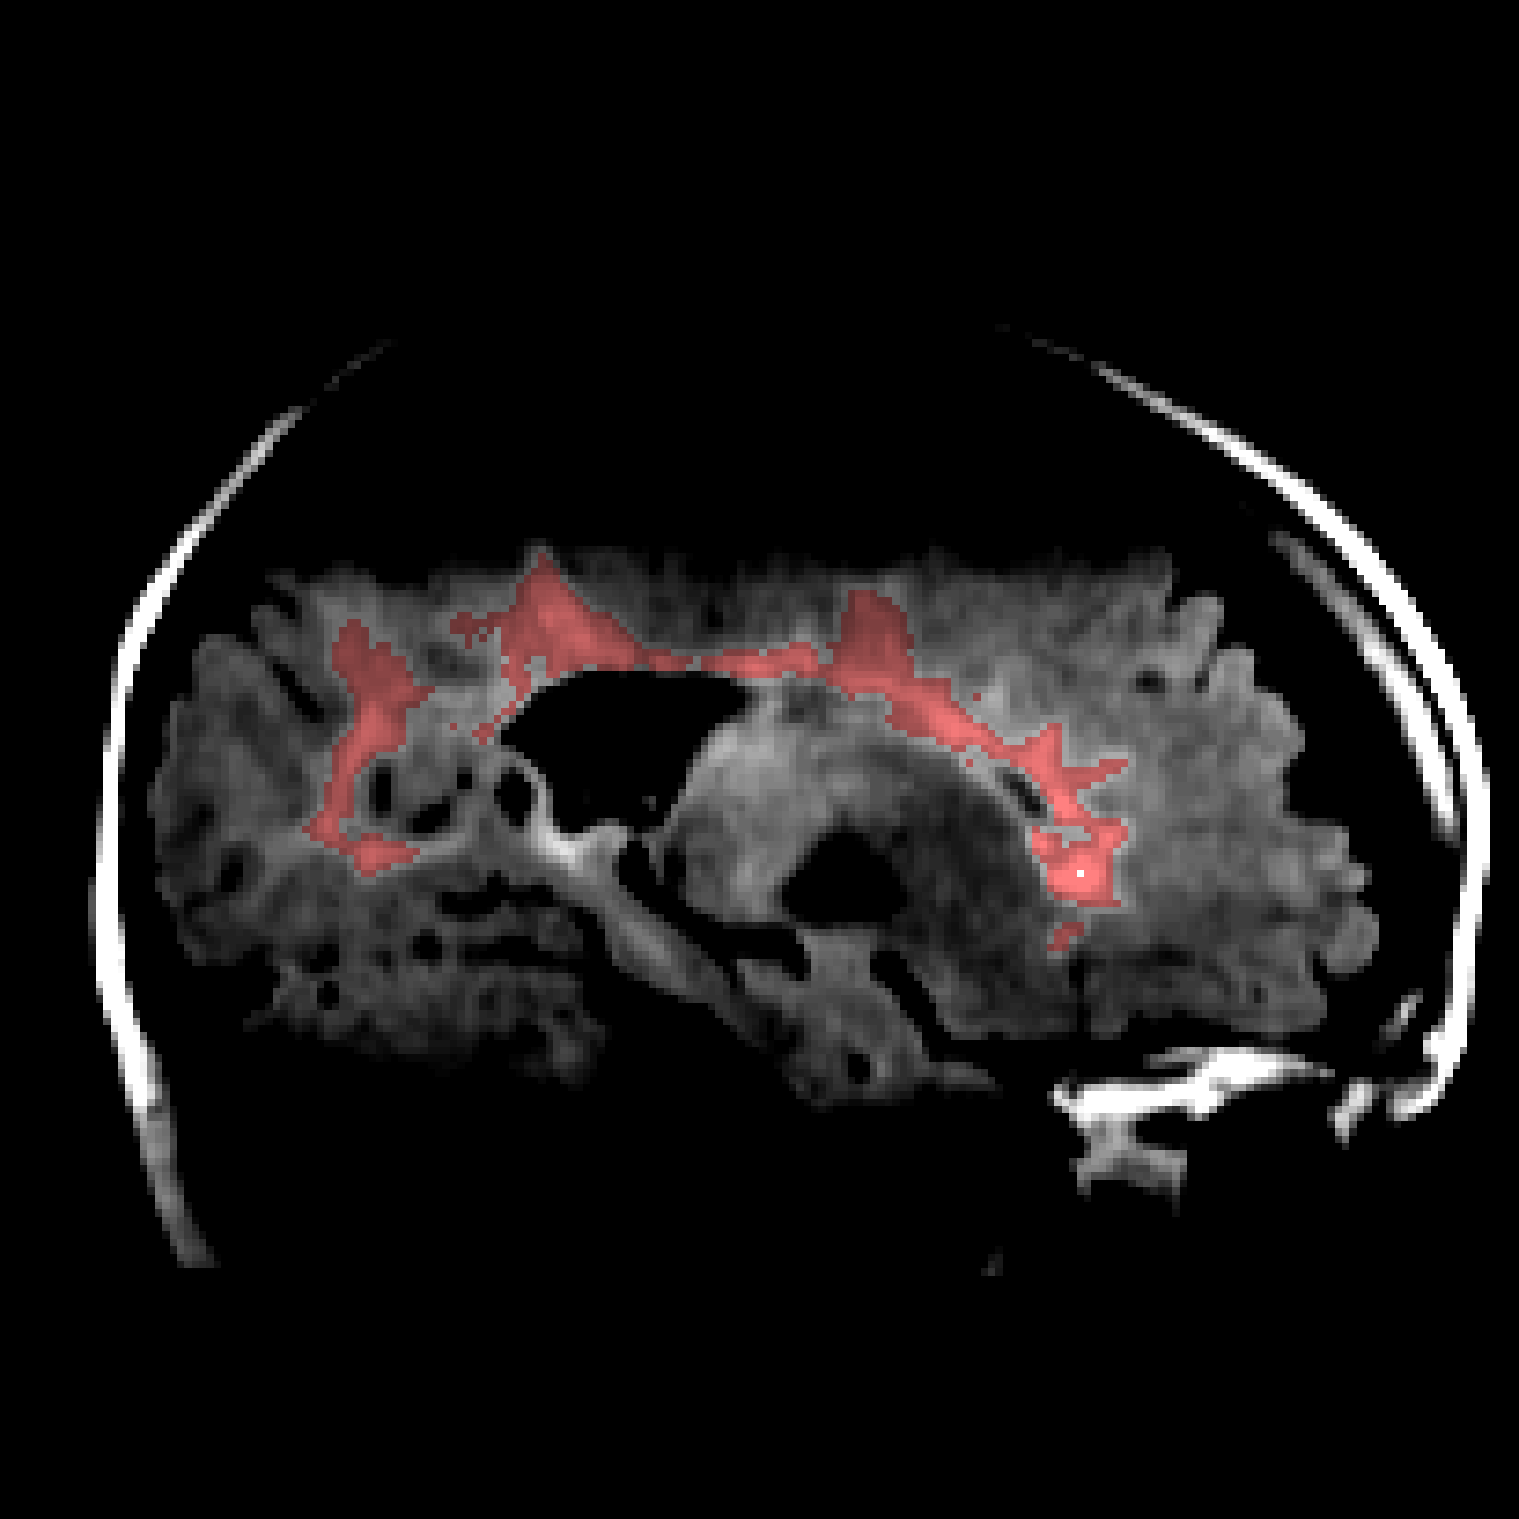
\includegraphics[height=6cm]{m08rev-01-d2-z146-r}\makebox[0pt][r]{\textcolor{white}{ CHB 01 }}\\[0.2em]
      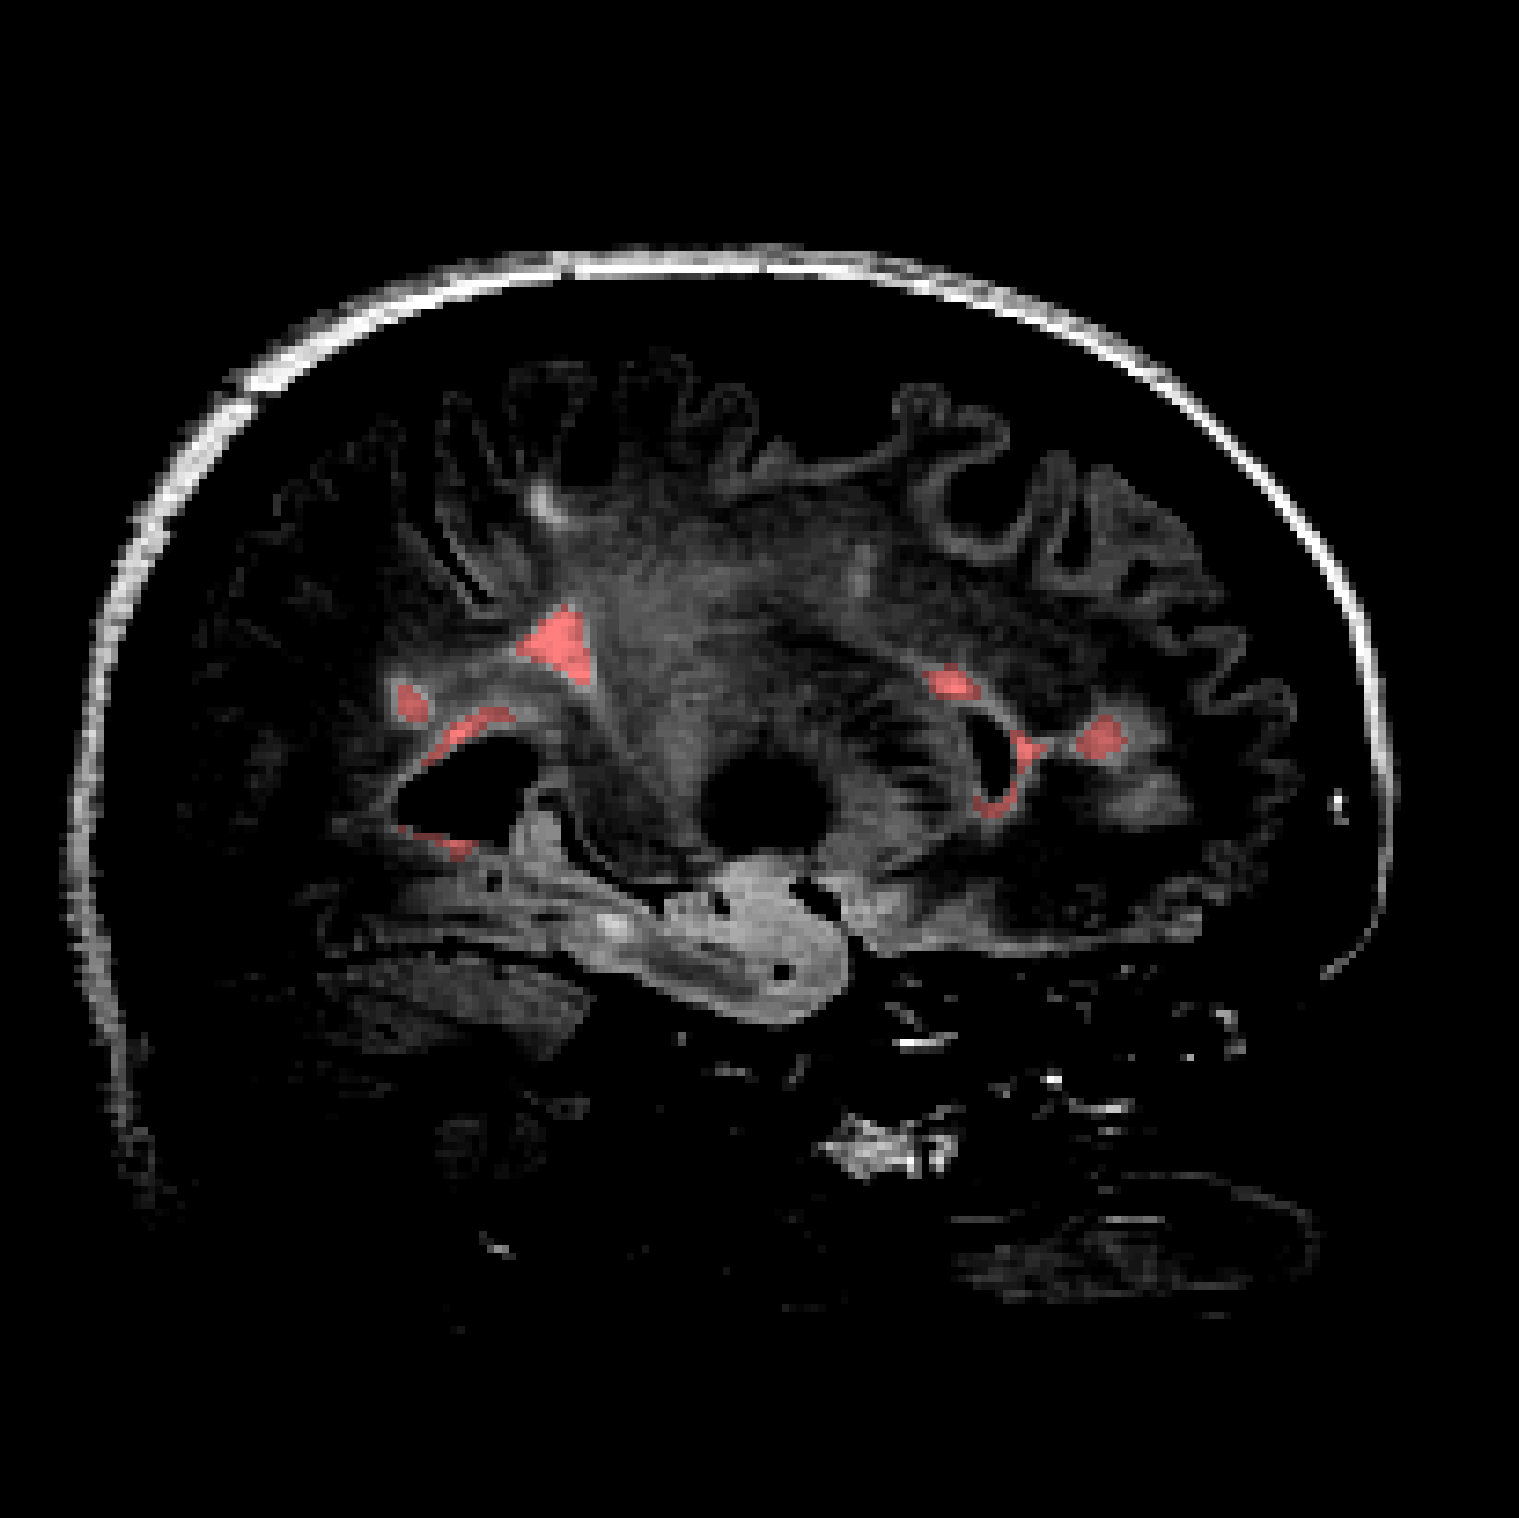
\includegraphics[height=6cm]{m08rev-05-d2-z107-r}\makebox[0pt][r]{\textcolor{white}{ CHB 05 }}\\[0.2em]
      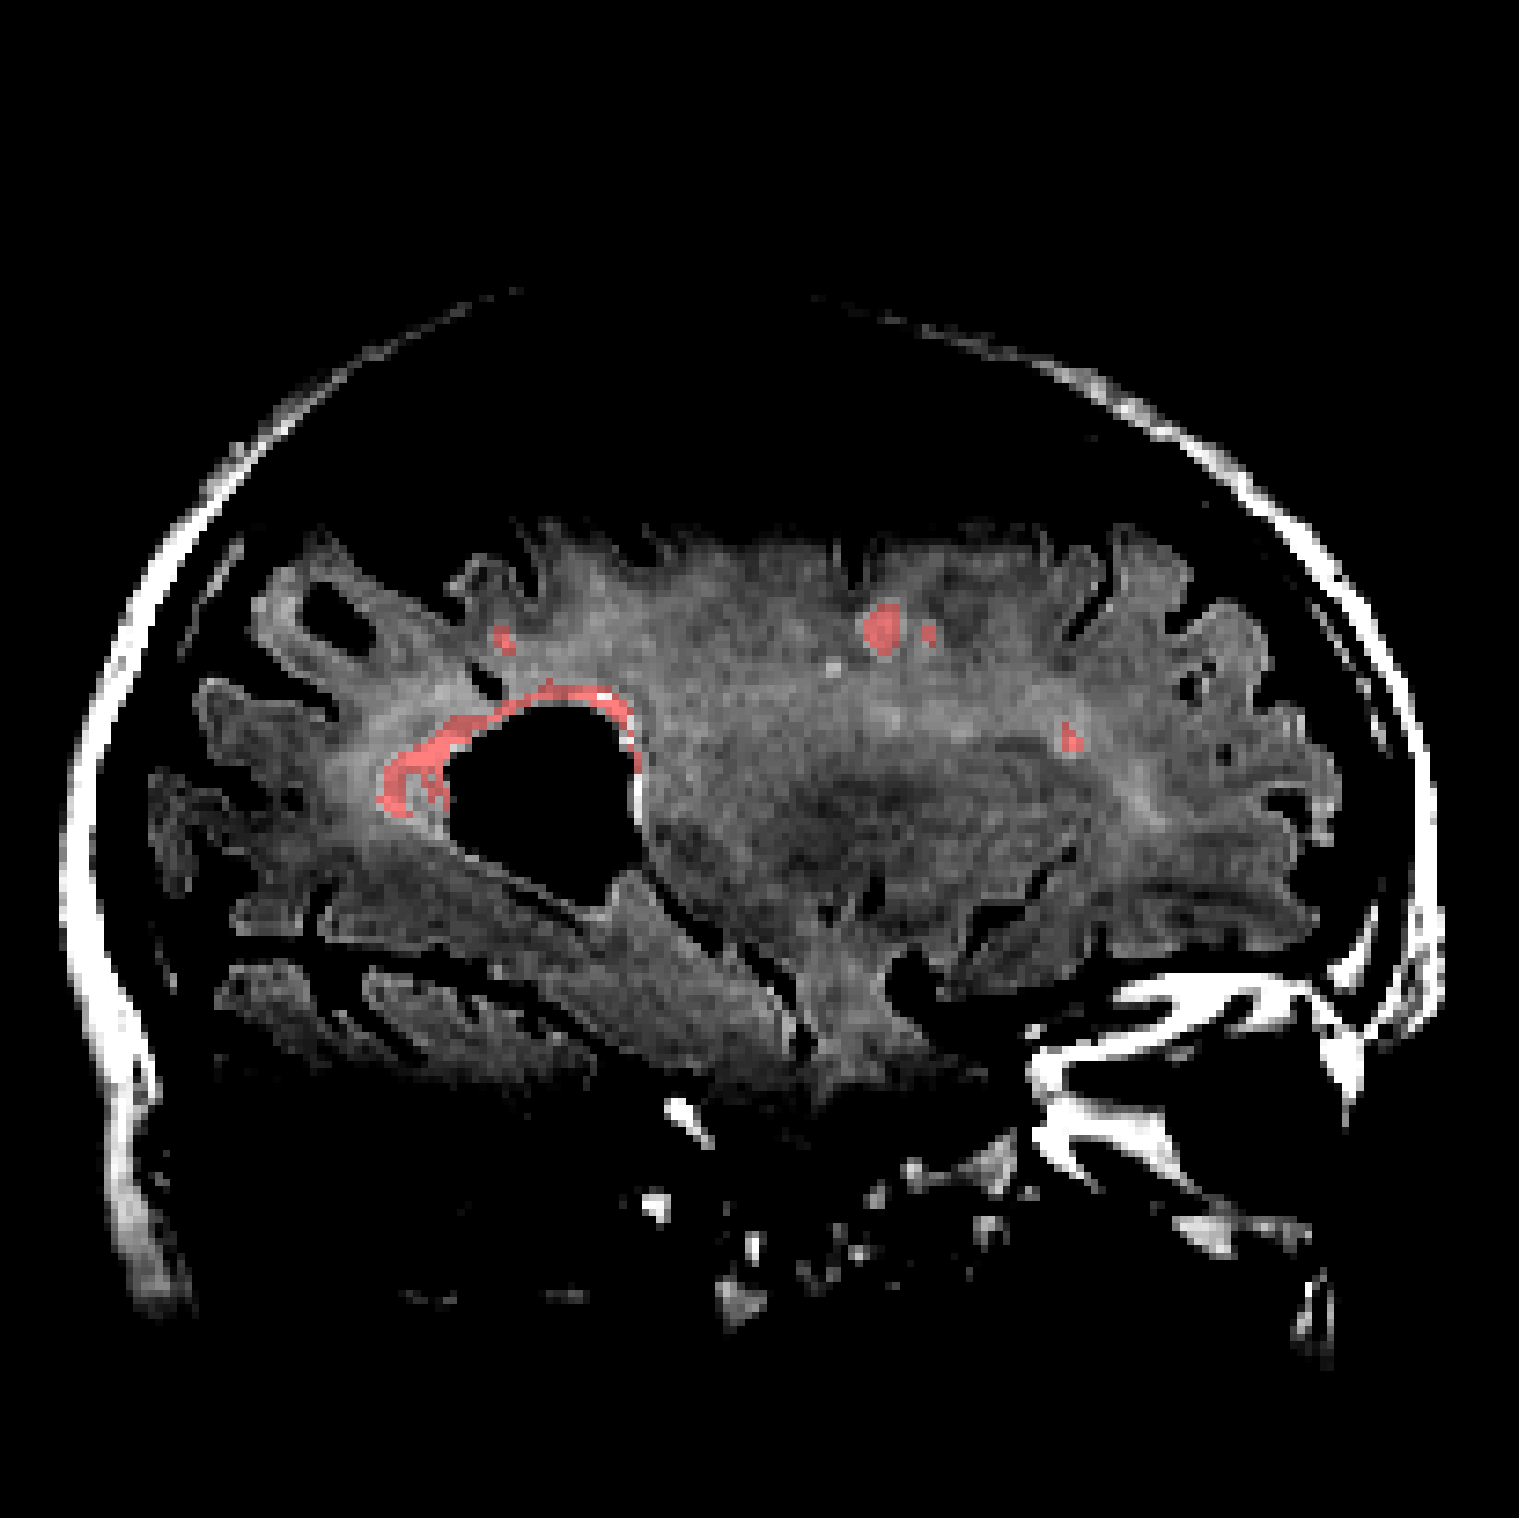
\includegraphics[height=6cm]{m08rev-06-d2-z101-r}\makebox[0pt][r]{\textcolor{white}{ CHB 06 }}
    \end{subfigure}
  \end{minipage}
  \caption{Example revisions to the manual segmentations for the MS 2008 challenge dataset.}
  \label{fig:m08-rev}
\end{figure}
% ==================================================================================================
\subsection{Brain Mask}\label{ss:brainmask}
In order to vectorize image data for parallel processing, a binary mask selecting voxels of interest in standardized space is also required. Since only voxels in the brain are of interest, this mask is called a ``brain mask''. The brain mask used here was derived from the ICBM tissue prior images \cite{Mazziotta2001} in MNI space: after initial thresholding of the combined $\gm+\wm+\csf$ probabilities at 0.5, manual refinements were completed and symmetry was enforced. The mask is slightly small on purpose, since tissues outside the brain are frequently bright in FLAIR images, and can be mistaken for lesions by naive models. The resulting mask is shown in Figure \ref{fig:brainmask}.
\begin{figure}
  \centering
  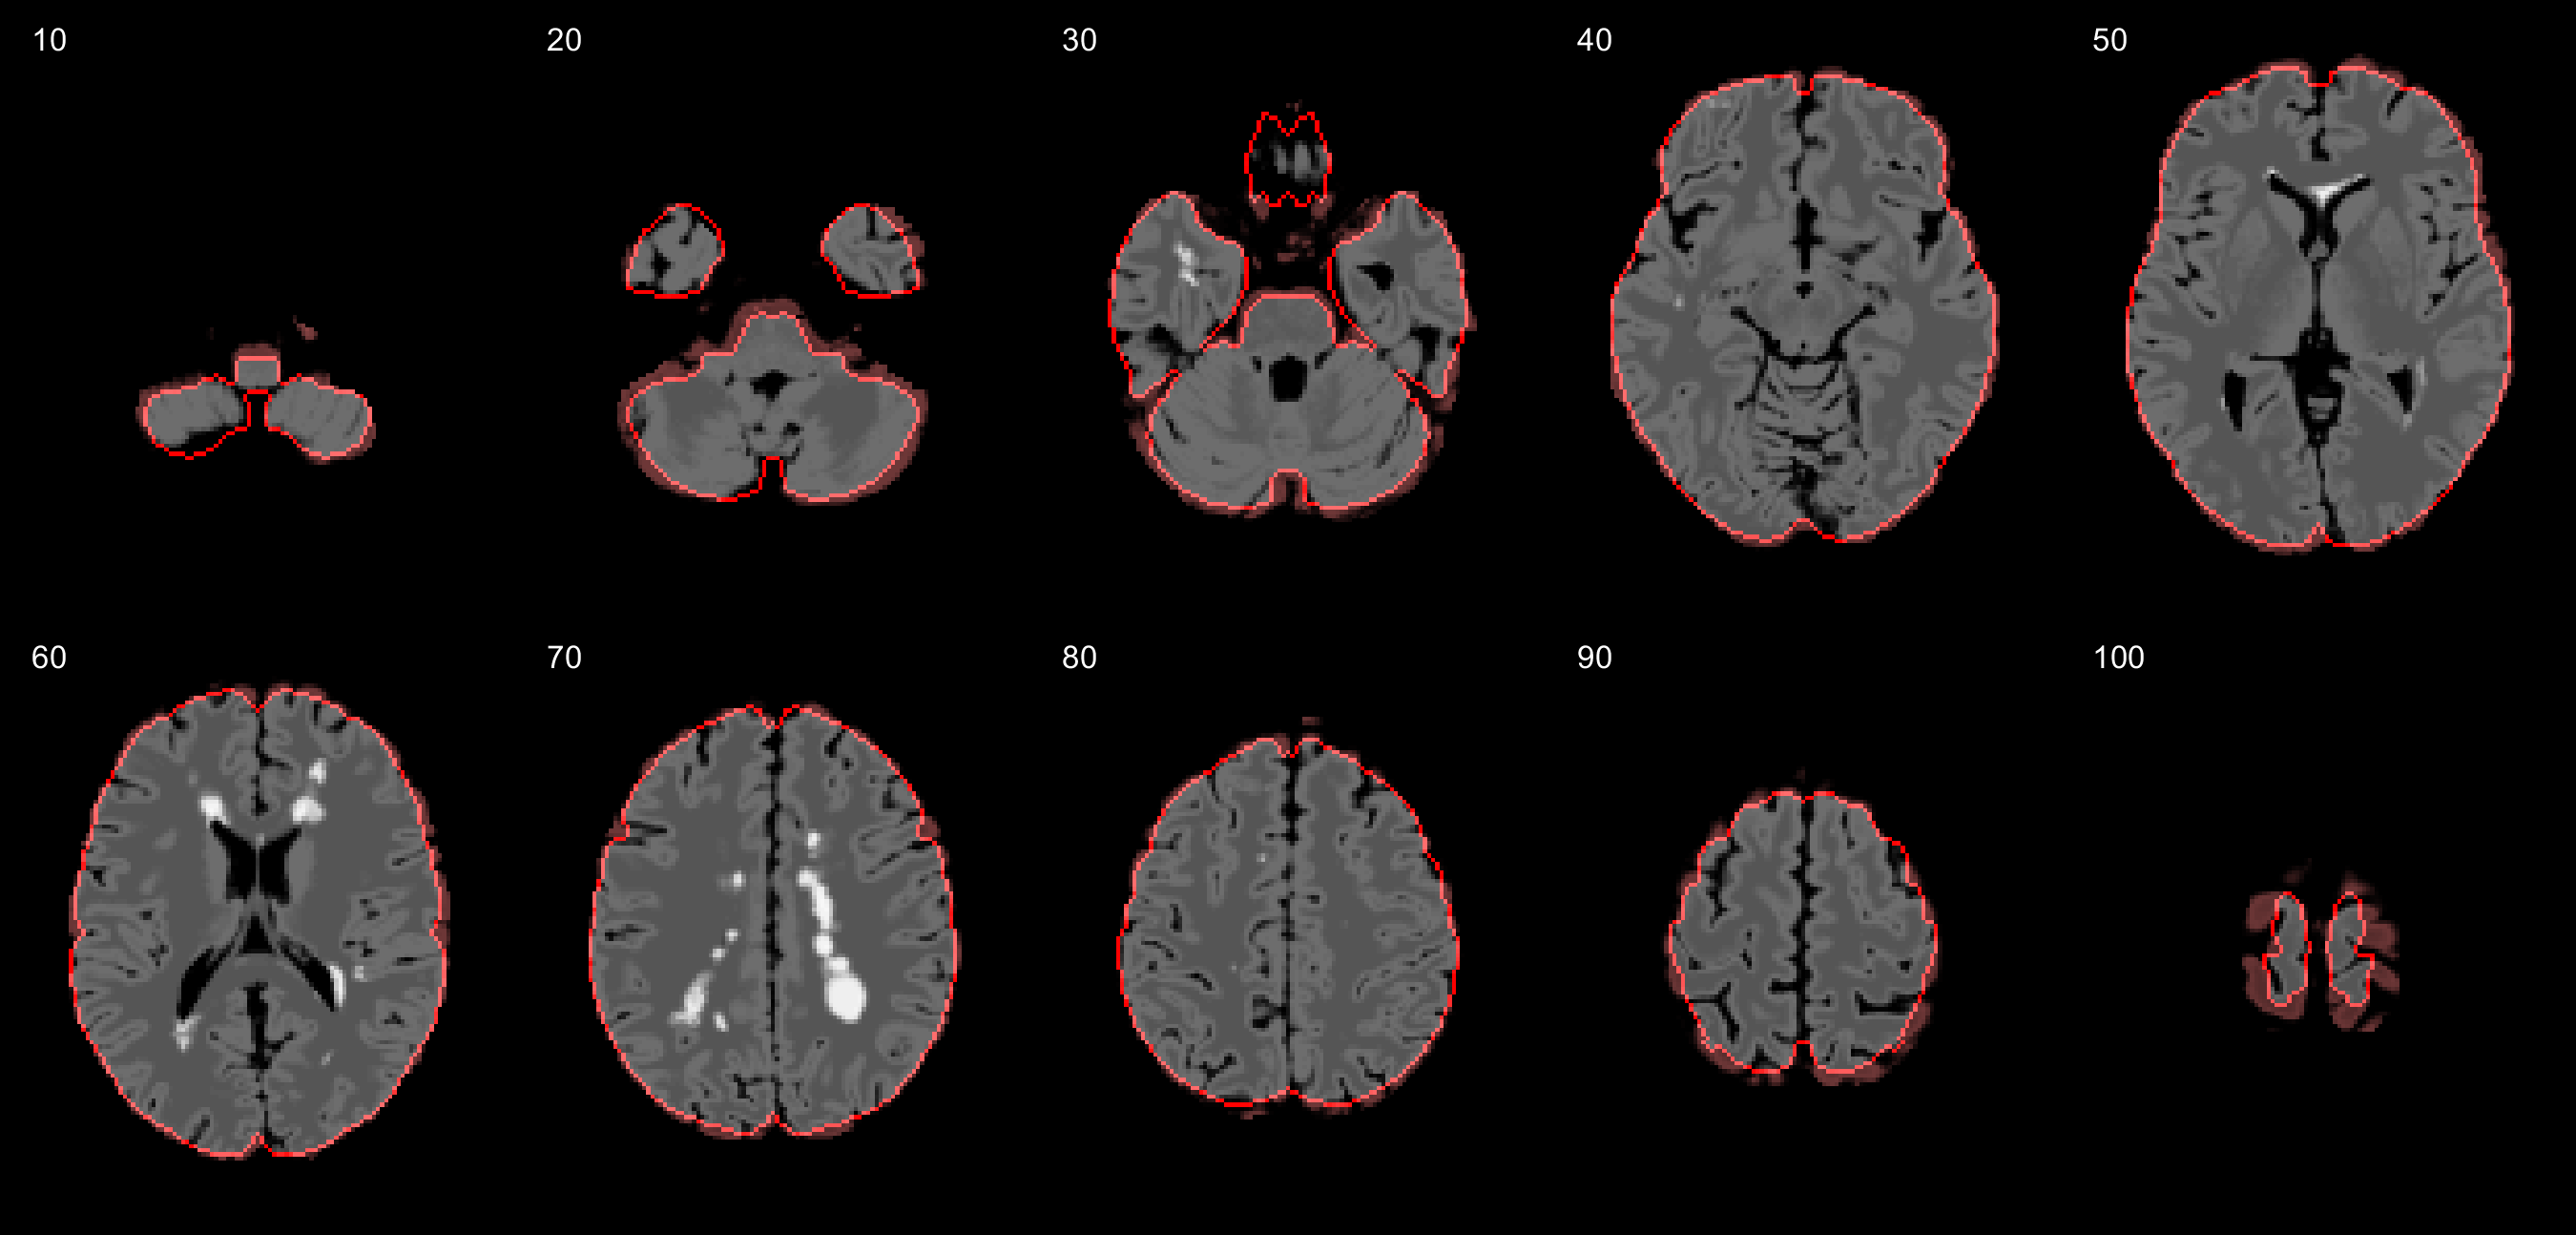
\includegraphics[height=2\sliceheight]{brainmask.png}
  \caption{Manually refined brain mask in MNI space. Mask outline is highlighted in red; inclusions are shown in grayscale; exclusions are tinted red.}
  \label{fig:brainmask}
\end{figure}
% --------------------------------------------------------------------------------------------------
% ==================================================================================================
%%%%%%%%%%%%%%%%%%%%%%%%%%%%%%%%%%%%%%%%%%%%%%%%%%%%%%%%%%%%%%%%%%%%%%%%%%%%%%%%%%%%%%%%%%%%%%%%%%%%
